% !TeX program = lualatex
\documentclass[11pt,a4paper]{article}

% ========= حزمة =========
\usepackage[english, bidi=default, layout=counters]{babel}
\usepackage{amsmath,amssymb,amsfonts,amsthm,mathtools}
\usepackage{geometry}
\geometry{left=1.25cm,right=1.25cm,top=1.25cm,bottom=3.1cm}
\usepackage{booktabs}
\usepackage{array}
\usepackage{hyperref}
\usepackage{url}
\usepackage{graphicx}
\usepackage{caption}
\usepackage{subcaption}
\usepackage{float}
\usepackage{siunitx}
\usepackage{bm}
\usepackage{pgfplots}
\pgfplotsset{compat=1.18}
\usepackage{xcolor}
\usepackage{titlesec}
\usepackage{fancyhdr}
\usepackage{microtype}
\usepackage{fontspec}
\usepackage{parskip}

% ========= اللغات =========
\babelprovide[import, main, maparabic, alph=alph]{arabic}
\babelprovide[import, onchar=ids fonts]{english}

% ========= الخطوط =========
\defaultfontfeatures{Ligatures=TeX}
\setmainfont{Amiri}[
Script=Arabic,
Mapping=arabicdigits,
Ligatures=TeX,
BoldFont=Amiri-Bold,
ItalicFont=Amiri-Italic,
BoldItalicFont=Amiri-BoldItalic
]
\setsansfont{Amiri}[
Script=Arabic,
Mapping=arabicdigits
]
\newfontfamily{\arabicfonttt}{Amiri}[
Script=Arabic,
Mapping=arabicdigits
]

% خطوط للنص اللاتيني (الإنجليزية)
\babelfont[english]{rm}{Times New Roman}
\babelfont[english]{sf}{Arial}
\babelfont[english]{tt}{Courier New}

% ========= ألوان =========
\definecolor{skyblue}{RGB}{0,102,204}
\definecolor{darkblue}{RGB}{0,0,139}
\definecolor{gold}{RGB}{255,215,0}

% ========= أوامر YUCT =========
\newcommand{\eps}{\varepsilon}
\newcommand{\kappac}{\kappa_c}
\newcommand{\Ke}{K_{\mathrm{eff}}}
\newcommand{\Keffi}[1]{K_{\mathrm{eff},#1}}
\newcommand{\betaf}{\beta}
\newcommand{\df}{d_{\!f}}
\newcommand{\Mpl}{M_{\mathrm{Pl}}}
\newcommand{\Lpl}{l_{\mathrm{Pl}}}
\newcommand{\tP}{t_{\mathrm{P}}}
\newcommand{\Sodd}{S_{\mathrm{odd}}}
\newcommand{\Seven}{S_{\mathrm{even}}}
\newcommand{\Dtau}{\Delta\tau_{\min}}
\newcommand{\Lzero}{L_0}
\newcommand{\alp}{\alpha}
\newcommand{\sigs}{\sigma}
\newcommand{\kb}{k_{\mathrm{B}}}
\newcommand{\Keffopt}{K_{\mathrm{eff},\mathrm{opt}}}
\newcommand{\Keffmax}{K_{\mathrm{eff},\max}}
\newcommand{\betac}{\beta}
\newcommand{\betagamma}{\beta\gamma}
\newcommand{\Scoord}{S_{\mathrm{coord}}}
\newcommand{\dint}{\ensuremath{D\!+\!I\!\cdot\!R}}
\newcommand{\RH}{R_{\mathrm{H}}}
\newcommand{\tH}{t_{\mathrm{H}}}
\newcommand{\ninf}{N_{\mathrm{e}}}
\newcommand{\ns}{n_{\mathrm{s}}}
\newcommand{\nt}{n_{\mathrm{T}}}
\newcommand{\rs}{r}
\newcommand{\alD}{\alpha_{\mathrm{D}}}
\newcommand{\beI}{\beta_{\mathrm{I}}}
\newcommand{\gaR}{\gamma_{\mathrm{R}}}
\newcommand{\Kcrit}{K_{\mathrm{crit}}}
\newcommand{\Rstruct}{R_{\mathrm{struct}}}
\newcommand{\Ntrials}{N_{\mathrm{trials}}}
\newcommand{\Nlife}{\langle N_{\mathrm{life}}\rangle}

% ========= عوامل =========
\DeclareMathOperator{\Var}{Var}
\DeclareMathOperator{\Cov}{Cov}
\DeclareMathOperator{\Div}{Div}
\DeclareMathOperator{\Grad}{Grad}
\DeclareMathOperator{\E}{\mathbb{E}}

% ========= نظريات =========
\newtheorem{theorem}{نظرية}[section]
\newtheorem{lemma}[theorem]{ليما}
\newtheorem{corollary}[theorem]{نتيجة}
\newtheorem{definition}[theorem]{تعريف}
\newtheorem{axiom}[theorem]{مسلّمة}
\newtheorem{proposition}[theorem]{اقتراح}
\newtheorem{remark}[theorem]{ملاحظة}
\newtheorem{hypothesis}[theorem]{فرضية}
\newtheorem{prediction}[theorem]{تنبؤ أعمى}

% ========= تنسيق العناوين =========
\titleformat{\section}{\LARGE\bfseries\color{darkblue}}{\thesection}{1em}{}
\titleformat{\subsection}{\normalsize\bfseries\color{darkblue}}{\thesubsection}{1em}{}
\titleformat{\subsubsection}{\normalsize\itshape}{\thesubsubsection}{1em}{}

% ========= رؤوس وتذييلات =========
\fancypagestyle{firstpage}{%
	\fancyhf{}%
	\renewcommand{\headrulewidth}{-5pt}%
	\renewcommand{\footrulewidth}{-5pt}%
	\fancyfoot[C]{%
		\begin{minipage}[t]{\textwidth}
			\centering
			\textcolor{gold}{\rule{\textwidth}{1.6pt}}\\[5pt]
			{\small \textsuperscript{1}أبحاث ياكوشيف، \url{https://yuct.org/}} \hfill
			{\small بروتوكول YPSDC: \url{https://ypsdc.com/}}\\[-2pt]
			\textcolor{gold}{\rule{\textwidth}{1.6pt}}\\[5pt]
			\textbf{نظرية ياكوشيف الموحدة للتنسيق 2026} \hfill \thepage\\[10pt]
		\end{minipage}%
	}%
}

\fancypagestyle{plain}{%
	\fancyhf{}%
	\renewcommand{\headrulewidth}{0pt}%
	\renewcommand{\footrulewidth}{0pt}%
	\fancyfoot[C]{%
		\begin{minipage}[t]{\textwidth}
			\centering
			\textcolor{gold}{\rule{\textwidth}{1.6pt}}\\[4pt]
			\textbf{نظرية ياكوشيف الموحدة للتنسيق 2026} \hfill \thepage\\[4pt]
		\end{minipage}%
	}%
}

\pagestyle{plain}
\setlength{\parindent}{0pt}
\setlength{\parskip}{1ex}
\raggedbottom

\hypersetup{
	colorlinks=true,
	linkcolor=blue,
	citecolor=blue,
	urlcolor=blue,
}

% ========= رأس المقال (YUCT logo) =========
\newcommand{\makeheader}{%
	\noindent
	\begin{minipage}{0.17\textwidth}
		\raggedright
		{\sffamily\bfseries\color{skyblue}\fontsize{46}{46}\selectfont YUCT}%
	\end{minipage}%
	\hspace{30pt}
	\begin{minipage}{0.32\textwidth}
		\raggedright
		{\sffamily\fontsize{11}{13}\selectfont نظرية ياكوشيف\\ الموحدة\\ للتنسيق}%
	\end{minipage}%
	\hfill
	\begin{minipage}{0.38\textwidth}
		\raggedleft
		{\sffamily\bfseries ملحق V}\\
		{\sffamily أبريل 2026}\\
		{\sffamily\footnotesize DOI: \url{https://doi.org/10.5281/zenodo.18444598}}%
	\end{minipage}
	\par\vspace{5pt}
	\noindent\textcolor{gold}{\rule{\textwidth}{1.6pt}}
	\par\vspace{0pt}
}

\begin{document}
	\thispagestyle{firstpage}
	\makeheader
	
	\vspace{0cm}
	
		{\LARGE\bfseries الزمن باعتباره إنتروبيا عمليات التنسيق: \\
			وصف موحد للزمن النسبي والثقالي والترموديناميكي في YUCT \par}
	
	\vspace{0.2cm}
	
	{\large أليكسي ف. ياكوشيف\footnote{أبحاث ياكوشيف، \url{https://yuct.org/}}} \\
	\vspace{0.0cm}
	
	{\color{darkblue}\textbf{\LARGE المستخلص}} \par
	{\large
		\noindent
		يقدم هذا الملحق تفسيراً جديداً للزمن في إطار نظرية ياكوشيف الموحدة للتنسيق (YUCT). يُعرَّف الزمن بأنه إنتروبيا عمليات التنسيق، مُقاساً بكفاءة التنسيق \(\Ke\). نُبيِّن أن عامل لورنتز \(\gamma\) في النسبية الخاصة وتباطؤ الزمن الثقالي في النسبية العامة ينبثقان طبيعياً كحالتين خاصتين من \(\Ke\). نشتق صيغة موحَّدة للزمن الخاص \(d\tau = dt/\Ke(v,\Phi)\) تختزل إلى الصيغ القياسية في الحدود المناسبة. بالنسبة للفوتون (\(v=c\))، \(\Ke \to \infty\) وينعدم الزمن الخاص، مما يُفسِّر لماذا لا يختبر الضوء زمناً. يؤدي تكميم إنتروبيا التنسيق إلى تكميم أساسي للزمن على مقياس بلانك، رابطاً ذلك بالجاذبية الكمومية. 
		
		نقوم بتوسيع الإطار ليشمل الثقوب السوداء، حيث نُبيِّن أن تقلُّبات الزمن تتدرج مع الكتلة وفق الأُس الشامل \(\beta = 0.67\). اللايقين النسبي في معدَّل الزمن يتدرج كـ \(\delta\tau/\tau \propto M^{-0.67}\)، مما يؤدِّي إلى تنبؤات قابلة للاختبار: (1) عرض التذبذبات شبه الدورية (QPOs) في أقراص تراكم الثقوب السوداء يجب أن يتدرج مع الكتلة كـ \(\Delta\nu/\nu \propto M^{-0.67}\)؛ (2) تشتت ترددات الرنين اللاحق (ringdown) للثقوب السوداء المندمجة يجب أن يتناقص مع الكتلة وفق نفس القانون. يمكن اختبار هذه التنبؤات ببيانات الأشعة السينية المتاحة (RXTE، NuSTAR) ورصد الموجات الثقالية (LIGO/Virgo، مرصد أينشتاين المستقبلي). يُوحِّد الإطار الجوانب النسبية والثقالية والترموديناميكية للزمن، مقدِّماً صورة متماسكة تتوافق مع قانون القياس الشامل \(\beta = 0.67\) (الملحق L) وديناميك تطور الأنظمة المعقدة (الملحق T).
	}
	
	\vspace{0.1cm}
	\noindent
	{\color{darkblue}\textbf{الكلمات المفتاحية:}} YUCT، الزمن، الإنتروبيا، كفاءة التنسيق، النسبية الخاصة، النسبية العامة، الثقب الأسود، QPO، ringdown، مقياس بلانك، الجاذبية الكمومية، تنبؤات تجريبية.
	
	\vspace{0.5cm}
	\noindent
	{\small نُسخة مختصرة من هذا العمل نُشرت سابقاً ومتاحة على \\ \url{https://doi.org/10.5281/zenodo.18362308}}
	\vspace{0.5cm}
	
	\noindent
	\textcopyright\ 2026 أبحاث ياكوشيف. جميع الحقوق محفوظة.
	
	\tableofcontents
	\newpage
	
	\section{مقدمة: مشكلة الزمن في الفيزياء الحديثة}
	\label{sec:intro}
	
	ظلَّت طبيعة الزمن أحد أعمق الألغاز في الفيزياء. ففي فروع مختلفة، يظهر الزمن بطرق مختلفة جوهرياً:
	\begin{itemize}
		\item في الميكانيك النيوتني، الزمن وسيط مطلق ومنتظم.
		\item في النسبية الخاصة، يصبح الزمن نسبياً ومتداخلاً مع المكان عبر تحويلات لورنتز.
		\item في النسبية العامة، الزمن ديناميكي ينحني بتأثير المادة والطاقة.
		\item في الترموديناميك، يرتبط الزمن بسهم تزايد الإنتروبيا.
		\item في ميكانيك الكم، يبقى الزمن وسيطاً خارجياً وليس مؤثراً.
	\end{itemize}
	
	توحي هذه الأدوار المتباينة بأن الزمن ليس أساسياً بل ناشئ عن مبدأ أعمق. تقترح نظرية ياكوشيف الموحدة للتنسيق (YUCT) أن التنسيق — العملية التي تُحاذي بها عناصر المنظومة حالاتها — هو الواقع الأولي. في هذا الملحق نُطوِّر فكرة أن \textbf{الزمن هو مقياس لإنتروبيا عمليات التنسيق}. يُوحِّد هذا التفسير طبيعياً الزمن النسبي والثقالي والترموديناميكي، ويُوفِّر جسراً نحو الجاذبية الكمومية عبر قانون القياس الشامل \(\beta = 0.67\) (الملحق L) وديناميك تطور الأنظمة المعقدة (الملحق T).
	
	الكمية الجوهرية في YUCT هي كفاءة التنسيق \(\Ke\)، المُعرَّفة كنسبة زمن التنسيق الساذج إلى زمن التنسيق الفعلي باستخدام قواميس موزَّعة مسبقاً (الملحق B). إنها تقيس مدى فعالية معالجة المنظومة للمعلومات ومزامنة مكوِّناتها. سنُبيِّن أن \(\Ke\) يرتبط مباشرةً بعامل لورنتز في النسبية الخاصة، وبعامل تباطؤ الزمن الثقالي في النسبية العامة، وبإنتاج الإنتروبيا في العمليات غير العكوسة. في حد الفوتون (\(v=c\))، \(\Ke \to \infty\) مما يعني أن الفوتون لا يختبر زمناً خاصاً — نتيجة تتوافق مع الجيوديسيات الصفرية في النسبية العامة ولكنها تكتسب الآن تفسيراً إنتروبياً.
	
	ثم نُوسِّع الإطار ليشمل الثقوب السوداء، حيث يصبح تداخل الكتلة ودرجة الحرارة والزمن جوهرياً. باستخدام قانون القياس الشامل، نشتق علاقة بين كتلة الثقب الأسود وتقلبات الزمن، مما يؤدِّي إلى تنبؤات قابلة للرصد فلكياً.
	
	\section{إنتروبيا التنسيق وعلاقتها بـ \(\Ke\)}
	\label{sec:coord_entropy}
	
	\subsection{تعريف إنتروبيا التنسيق}
	
	لنعتبر لمنظومة مجموعة من حالات التنسيق الممكنة \(\{C_i\}\) باحتمالات \(p_i\). بالإضافة إلى ذلك، تمتلك المنظومة قواميس \(D_j\) (مجموعات منظمة من البروتوكولات أو القواعد أو الأنماط) مع كفاءات تنسيق مرتبطة بها \(\Keffi{j}\). تُعرَّف إنتروبيا التنسيق الكلية كالآتي:
	\begin{equation}
		\Scoord = -k_B \sum_{i=1}^{N} p_i \ln p_i \;+\; k_B \sum_{j=1}^{M} \Keffi{j} \ln D_j.
		\label{eq:coord_entropy_def}
	\end{equation}
	الحد الأول هو إنتروبيا شانون لاحتمالات الحالات؛ أما الحد الثاني فيُمثِّل المعلومات المخزَّنة في القواميس، مُثقَّلة بكفاءتها. يعكس العامل \(\Keffi{j} \ln D_j\) حقيقة أن القاموس الأكثر كفاءة (أعلى \(\Ke\)) يُساهم بشكل أكبر في قدرة المنظومة على توليد أنماط منسَّقة.
	
	\subsection{العلاقة بالمعلومات وقياس الخطأ}
	
	من قانون الخطأ الشامل (الملحق L)،
	\begin{equation}
		\varepsilon = \kappac \alpha \Ke^{-\beta}, \quad \beta = 0.67,\ \kappac = 0.33,
	\end{equation}
	يُمثِّل الخطأ النسبي \(\varepsilon\) نسبة التنسيقات غير الناجحة. كمية المعلومات المُعالَجة بنجاح في وحدة الزمن تتناسب مع \(\Ke\). ومن ثم، يمكن كتابة تغير إنتروبيا التنسيق خلال فترة زمنية صغيرة على النحو:
	\begin{equation}
		d\Scoord = k_B \ln 2 \cdot dI = k_B \ln 2 \cdot \frac{d\mathcal{A}}{\langle \mathcal{A} \rangle},
	\end{equation}
	حيث \(I\) هي المعلومات بالبتات و\(\mathcal{A}\) هو عدد الأفعال المنسَّقة الناجحة. في الحد المتصل، يؤدي هذا إلى تناسب بين معدل تغير \(\Scoord\) و\(\Ke\) نفسه.
	
	\subsection{المسلَّمة الأساسية}
	
	\begin{axiom}[الزمن باعتباره إنتروبيا التنسيق]
		مرور الزمن الخاص \(\tau\) على طول خط عالمي لمنظومة يتناسب طرداً مع تغير إنتروبيا تنسيقها:
		\begin{equation}
			d\tau = \frac{1}{\beta_0} \, d\Scoord,
			\label{eq:time_entropy}
		\end{equation}
		حيث \(\beta_0\) ثابت كوني بأبعاد إنتروبيا لكل زمن. سيتم ربط هذا الثابت بوحدات بلانك في القسم \ref{sec:quantization}.
	\end{axiom}
	
	تُعرِّف هذه المسلَّمة تدفق الزمن بتزايد إنتروبيا التنسيق. وهي تعني أن أية منظومة ذات إنتروبيا تنسيق ثابتة (مثلاً فوتون في الخلاء) لا تختبر زمناً — إنها "مجمَّدة" في حالة لازمانية.
	
	\section{تباطؤ الزمن النسبي كنتيجة لـ \(\Ke\)}
	\label{sec:sr}
	
	\subsection{\(\Ke\) كعامل لورنتز}
	
	بالنسبة لمنظومة تتحرك بسرعة \(v\) بالنسبة لمراقب، تكتسب كفاءة التنسيق مساهمة حركية. في النسبية الخاصة، يقيس عامل لورنتز \(\gamma = (1-v^2/c^2)^{-1/2}\) مدى تباطؤ زمن الإطار المتحرك. نقترح:
	\begin{definition}[\(\Ke\) النسبوي]
		\[
		\Ke(v) = \gamma(v) = \frac{1}{\sqrt{1-\dfrac{v^2}{c^2}}}.
		\]
	\end{definition}
	
	\begin{theorem}[تباطؤ الزمن في النسبية الخاصة]
		يرتبط عنصر الزمن الخاص \(d\tau\) بالزمن الإحداثي \(dt\) بالعلاقة
		\begin{equation}
			d\tau = \frac{dt}{\Ke(v)} = dt\sqrt{1-\frac{v^2}{c^2}}.
		\end{equation}
	\end{theorem}
	
	\begin{proof}
		من المسلَّمة \ref{eq:time_entropy}، \(d\tau = d\Scoord/\beta_0\). يمكن حساب تغير إنتروبيا التنسيق لمنظومة متحركة من تزايد عدد الحالات الممكنة بفعل الحركة. باستخدام التعريف (\ref{eq:coord_entropy_def}) وحقيقة أن عدد القواميس المتاحة يتزايد مع السرعة، نجد \(d\Scoord \propto \gamma(v)\, dt\). يُمتص ثابت التناسب في \(\beta_0\) وينشأ العامل \(1/\gamma\) من الفاصلة اللامتباينة.
	\end{proof}
	
	وهكذا يُعاد تفسير تباطؤ الزمن المألوف في النسبية الخاصة على أنه نقصان في معدل تزايد الإنتروبيا عند الرصد من إطار متحرك.
	
	\section{تباطؤ الزمن الثقالي}
	\label{sec:gr}
	
	في حقل ثقالي ضعيف بكمون \(\Phi = -GM/r\)، تُعطي المترية عنصر الزمن الخاص
	\begin{equation}
		d\tau = dt\sqrt{1 + \frac{2\Phi}{c^2}} \approx dt\left(1 + \frac{\Phi}{c^2}\right).
	\end{equation}
	
	\begin{definition}[\(\Ke\) الثقالي]
		لمنظومة ساكنة في كمون ثقالي \(\Phi\)،
		\[
		\Ke(\Phi) = \frac{1}{\sqrt{1 + \dfrac{2\Phi}{c^2}}}.
		\]
	\end{definition}
	
	\begin{theorem}[تباطؤ الزمن الثقالي]
		\begin{equation}
			d\tau = \frac{dt}{\Ke(\Phi)} = dt\sqrt{1 + \frac{2\Phi}{c^2}}.
		\end{equation}
	\end{theorem}
	
	\begin{proof}
		في حقل ثقالي، تزداد كفاءة التنسيق لأن الكمون يركِّز الحالات المتاحة (مثلاً بانحناء الزمكان). يؤدي هذا إلى معدل أعلى لإنتاج الإنتروبيا، مما يعني وفق المسلَّمة \ref{eq:time_entropy} تباطؤاً في الزمن الخاص. يتبع العامل الدقيق من مترية شفارتسشيلد في حد الحقل الضعيف.
	\end{proof}
	
	\section{تعبير موحَّد للزمن الخاص}
	\label{sec:unified}
	
	بدمج مساهمتي السرعة والجاذبية نحصل على:
	
	\begin{theorem}[\(\Ke\) العام والزمن الخاص]
		لمنظومة تتحرك بسرعة \(v\) في كمون ثقالي ضعيف \(\Phi\)، تكون كفاءة التنسيق الكلية
		\begin{equation}
			\Ke(v,\Phi) = \frac{1}{\sqrt{1 + \dfrac{2\Phi}{c^2} - \dfrac{v^2}{c^2}}}.
		\end{equation}
		وعنصر الزمن الخاص هو
		\begin{equation}
			d\tau = \frac{dt}{\Ke(v,\Phi)} = dt\sqrt{1 + \frac{2\Phi}{c^2} - \frac{v^2}{c^2}}.
		\end{equation}
	\end{theorem}
	
	\begin{proof}
		لنأخذ مترية شفارتسشيلد في تقريب الحقل الضعيف:
		\[
		ds^2 = \left(1+\frac{2\Phi}{c^2}\right)c^2 dt^2 - \left(1-\frac{2\Phi}{c^2}\right)(dx^2+dy^2+dz^2).
		\]
		للحركة على طول المحور \(x\) بسرعة \(v = dx/dt\)،
		\[
		ds^2 = c^2 dt^2\left[ \left(1+\frac{2\Phi}{c^2}\right) - \left(1-\frac{2\Phi}{c^2}\right)\frac{v^2}{c^2} \right].
		\]
		بإبقاء الحدود من الرتبة الأولى فقط في \(\Phi/c^2\) و\(v^2/c^2\)، يُصبح القوس
		\[
		1 + \frac{2\Phi}{c^2} - \frac{v^2}{c^2} + \mathcal{O}\left(\frac{\Phi v^2}{c^4}\right).
		\]
		ثم \(d\tau = ds/c = dt\sqrt{1 + 2\Phi/c^2 - v^2/c^2}\). بتعريف \(\Ke = 1/\sqrt{1 + 2\Phi/c^2 - v^2/c^2}\) نحصل على العلاقة المطلوبة.
	\end{proof}
	
	تُوحِّد هذه الصيغة تأثيري تباطؤ الزمن الكلاسيكيين تحت المفهوم الوحيد لكفاءة التنسيق. كما تُظهر أنه بالنسبة للفوتون (\(v=c\), \(\Phi=0\))، \(\Ke \to \infty\) و\(d\tau = 0\)، مما يؤكد أن الضوء لا يختبر زمناً خاصاً — خطه العالمي معدوم.
	
	\section{الزمن كإنتروبيا: علاقات كمية}
	\label{sec:entropy}
	
	من المسلَّمة \ref{eq:time_entropy} وتعريف \(\Ke\)، يمكننا اشتقاق علاقة مباشرة بين معدَّل الزمن الخاص و\(\Ke\).
	
	\begin{theorem}[إنتاج الإنتروبيا و\(\Ke\)]
		\[
		\frac{d\Scoord}{d\tau} = \beta_0.
		\]
		أي أن معدل تزايد إنتروبيا التنسيق بالنسبة للزمن الخاص ثابت. أما بالنسبة للزمن الإحداثي،
		\[
		\frac{d\Scoord}{dt} = \frac{\beta_0}{\Ke}.
		\]
	\end{theorem}
	
	تعني هذه النتيجة أن الساعة تقيس تراكم إنتروبيا التنسيق. في منظومة متحركة أو متأثرة بالجاذبية، تكون \(\Ke\) أكبر، فتتزايد الإنتروبيا أبطأ بالنسبة للزمن الإحداثي — ومن ثم يتباطأ الزمن.
	
	\subsection{الارتباط بالقانون الثاني}
	
	ينص القانون الثاني للترموديناميك على أن الإنتروبيا الكلية لمنظومة معزولة لا تتناقص أبداً. في إطارنا، يصبح هذا:
	\begin{equation}
		\frac{d\Scoord}{d\tau} \ge 0.
	\end{equation}
	وهكذا يُحدَّد سهم الزمن بتزايد إنتروبيا التنسيق. العمليات غير العكوسة هي التي تزيد \(\Scoord\)؛ والعمليات العكوسة تُبقيها ثابتة. في حد التنسيق المثالي (\(\Ke \to \infty\))، يتوقف إنتاج الإنتروبيا وتصبح المنظومة لازمانية (مثلاً الفوتون).
	
	\section{تكميم الزمن ومقياس بلانك}
	\label{sec:quantization}
	
	إن إنتروبيا التنسيق \(\Scoord\) ليست كمية متصلة؛ إنها مبنية من بتات متقطعة من المعلومات. يوحي هذا بتقطُّع أساسي.
	
	\begin{hypothesis}[تكميم إنتروبيا التنسيق]
		تتغير إنتروبيا التنسيق بخطوات متقطعة:
		\begin{equation}
			\Delta \Scoord = n \cdot S_0, \quad n \in \mathbb{N},
		\end{equation}
		حيث \(S_0 = k_B \ln 2\) هي الإنتروبيا المقابلة لبت واحد من المعلومات.
	\end{hypothesis}
	
	من المسلَّمة \ref{eq:time_entropy}، يعني هذا بنية متقطعة للزمن الخاص:
	\begin{equation}
		\Delta \tau = \frac{S_0}{\beta_0}.
	\end{equation}
	
	يمكن التعبير عن الثابت \(\beta_0\) بوحدات بلانك. في الملحق L، ترتبط إنتروبيا التنسيق الصغرى بالبنية الثلاثية D+I•R، مما يُعطي \(\kappac = e^{-S_{\min}/k_B} = 1/3\). بالنسبة لمقياس بلانك، نتوقع أن تكون \(\beta_0\) من رتبة \(k_B / t_P\)، حيث \(t_P\) هو زمن بلانك. بدقة أكبر، يُعطي التحليل البُعدي:
	\begin{equation}
		\beta_0 = \frac{k_B c}{\Lpl} = k_B \cdot \frac{c}{\Lpl},
	\end{equation}
	حيث \(\Lpl = \sqrt{\hbar G/c^3}\) هي طول بلانك. وعندئذٍ
	\begin{equation}
		\Delta \tau_{\min} = \frac{S_0}{\beta_0} = \frac{\ln 2 \cdot \Lpl}{c} = \ln 2 \cdot t_P \approx 0.693 \, t_P.
	\end{equation}
	وهكذا، الزمن مُكمَّم بوحدات من زمن بلانك، بما يتوافق مع توقعات الجاذبية الكمومية.
	
	\section{تدرج الثقوب السوداء وتنبؤات عمياء}
	\label{sec:blackhole}
	
	تُوفِّر الثقوب السوداء مختبراً طبيعياً لاختبار تدرج تقلبات الزمن مع الكتلة. حجمها المميز هو نصف القطر الثقالي \(R_g = 2GM/c^2\)، الذي يُمثِّل مقياس الطول الأساسي للمنظومة. في YUCT، يجب أن تتدرج كفاءة التنسيق \(\Ke\) لثقب أسود مع كتلته. تدعم هذا عدة خطوط استدلالية:
	\begin{itemize}
		\item درجة حرارة هوكينغ \(T_H \propto 1/M\) تُشير إلى أن الثقوب السوداء الأكثر كتلة أبرد وأكثر ترتيباً، مما يعني \(\Ke\) أعلى.
		\item إنتروبيا بيكنشتاين–هوكينغ \(S_{\text{BH}} = k_B A/(4\ell_P^2) \propto M^2\) تُظهر أن المحتوى المعلوماتي ينمو مع المساحة لا الحجم، مما يوحي بأن التنسيق مُشفَّر على الأفق.
		\item يتدرج زمن التبخر كـ \(t_{\text{ev}} \propto M^3\)، أي أن الثقوب السوداء الأكبر تعيش أطول بكثير.
	\end{itemize}
	بهذه الدلائل، نفترض قانون قوة بسيطاً:
	\begin{equation}
		\Ke(M) \propto M^{\alpha}, \quad \alpha \approx 1,
	\end{equation}
	حيث يمكن تحديد الأُس الدقيق بأعمال نظرية لاحقة. لغرض وضع تنبؤات قابلة للاختبار، نعتمد \(\alpha = 1\) كأبسط افتراض.
	
	من قانون القياس الشامل \(\delta \tau / \tau \propto \Ke^{-\beta}\) مع \(\beta = 0.67\)، نحصل على العلاقة المركزية:
	\begin{equation}
		\boxed{\frac{\delta \tau}{\tau} \propto M^{-0.67}}.
	\end{equation}
	وهكذا، يتناقص التذبذب النسبي (اللايقين) في معدَّل الزمن الخاص مع تزايد كتلة الثقب الأسود كقانون قوة بأُس \(-0.67\).
	
	\subsection{التنبؤ 1: التذبذبات شبه الدورية (QPOs)}
	
	تُظهر الثقوب السوداء المتراكمة تذبذبات شبه دورية في تدفق أشعتها السينية. تتناسب ترددات هذه QPOs عكسياً مع الكتلة: \(\nu \propto 1/M\). عرضها النسبي \(\Delta\nu/\nu\) هو مقياس لاستقرار التدفق التراكمي الداخلي. إذا كان الزمن نفسه يتذبذب، فستنطبع هذه التذبذبات على عرض QPO. يتنبأ نموذجنا:
	\begin{prediction}[تدرج عرض QPO]
		يجب أن يتدرج العرض الكسري لقمم QPO مع كتلة الثقب الأسود كـ
		\begin{equation}
			\frac{\Delta\nu}{\nu} \propto M^{-0.67}.
		\end{equation}
		يمكن اختبار هذا بمقارنة بيانات QPO من ثقوب سوداء نجمية (رُصدت بـ RXTE، NICER، Insight-HXMT) وثقوب سوداء فائقة الكتلة (رُصدت بـ XMM-Newton، NuSTAR، ومهمات مستقبلية مثل Athena).
	\end{prediction}
	
	\subsection{التنبؤ 2: تشتت الرنين اللاحق في الموجات الثقالية}
	
	عند اندماج ثقبين أسودين، يُصدر الثقب الأسود الناتج موجات ثقالية رنينية لاحقة (ringdown) — تراكب من الجيوب المضمحلة بترددات وأزمنة اضمحلال تُحدِّدها كتلته وزمخه. يتدرج تردد النمط الأساسي \(\omega\) كـ \(1/M\). يجب أن يعكس تشتت الكتلة المُستنتَجة من أحداث رنين لاحق متعددة (أو من النغمات الفوقية في حدث واحد) التذبذبات الكامنة للزمن. يتنبأ نموذجنا:
	\begin{prediction}[تشتت الرنين اللاحق]
		تشتت تردد الرنين اللاحق المقيس (أو الكتلة) لعينة من الثقوب السوداء يجب أن يتناقص مع الكتلة كـ \(\sigma_{\omega}/\omega \propto M^{-0.67}\). يمكن اختبار هذا بفهارس الموجات الثقالية من LIGO/Virgo/KAGRA (الحالية والمستقبلية) وفي النهاية بمرصد أينشتاين و Cosmic Explorer.
	\end{prediction}
	
	\subsection{الارتباط بالاعتماد على درجة الحرارة}
	
	تتناسب درجة حرارة الثقب الأسود عكسياً مع كتلته، \(T_H \propto 1/M\). بدمج هذا مع تدرجنا \(\delta\tau/\tau \propto M^{-0.67}\) نحصل على علاقة مكافئة بدلالة درجة الحرارة:
	\begin{equation}
		\frac{\delta\tau}{\tau} \propto T_H^{0.67}.
	\end{equation}
	يتوافق هذا مع اعتماد الجاذبية على درجة الحرارة الموجود في الملحق P (\(\beta\gamma = 0.20\))، لأن تقلبات الزمن هي تجلٍ مباشر أكثر لنفس الفيزياء الأساسية.
	
	\section{أزمنة التفاعلات الكيميائية: منظور تنسيقي}
	\label{sec:chemistry}
	
	يجد مفهوم الزمن كمقياس لإنتروبيا التنسيق تطبيقاً طبيعياً في الحركية الكيميائية. الزمن اللازم لحدوث تفاعل كيميائي، المُعبَّر عنه عادةً بثابت المعدَّل \(k(T)\)، ليس مجرد دالة لطاقة التنشيط ودرجة الحرارة، بل أيضاً لكفاءة تنسيق الجزيئات المتفاعلة وبيئتها. في YUCT، يُعطى ثابت المعدَّل بمعادلة أرينيوس–ياكوشيف (الملحق C، معادلة \ref{eq:arrhenius-yakushev}):
	
	\begin{equation}
		k(T) = A \exp\left[-\frac{E_a}{RT} - \lambda \left(\frac{T}{T_0}\right)^{\beta\gamma}\right], \quad \beta\gamma = 0.20,
	\end{equation}
	
	حيث يعكس الحد الإضافي \(-\lambda (T/T_0)^{\beta\gamma}\) تأثير كفاءة التنسيق على معدَّل التفاعل. ينشأ هذا الحد لأن كفاءة التنسيق \(\Ke(T)\) تتناقص مع تزايد درجة الحرارة، وفقاً لـ \(\Ke(T) \propto T^{-\gamma}\) (الملحق P). لذلك، يتدرج زمن التفاعل \(\tau_{\mathrm{reaction}} = 1/k(T)\) كـ
	
	\begin{equation}
		\tau_{\mathrm{reaction}} \propto \exp\left[\lambda \left(\frac{T}{T_0}\right)^{\beta\gamma}\right] \propto \Ke(T)^{-\beta},
	\end{equation}
	
	لأن \(\Ke(T)^{-\beta} \propto T^{\beta\gamma}\) والأسي هو المسيطر. هذا تجلٍ مباشر لقانون القياس الشامل \(\delta \tau / \tau \propto \Ke^{-\beta}\) مُطبَّقاً على العمليات الكيميائية.
	
	من المنظور الإنتروبي (القسم \ref{sec:entropy})، يُمثِّل تقدُّم التفاعل الكيميائي تزايداً في إنتروبيا التنسيق \(\Scoord\) كلما انتقلت المنظومة من متفاعلات منتظمة إلى نواتج أكثر اضطراباً. الزمن الخاص \(\tau\) الذي تختبره الجزيئات المتفاعلة يتناسب مع تراكم هذه الإنتروبيا، \(d\tau = d\Scoord / \beta_0\). يتحكم \(\Ke\) بمعدَّل إنتاج الإنتروبيا، ومن ثم بمعدَّل التفاعل: كفاءة تنسيق أعلى (مثلاً بوجود حفَّاز) تؤدي إلى تزايد أسرع للإنتروبيا وبالتالي زمن تفاعل أقصر.
	
	يُوحِّد هذا الإطار الحركية الكيميائية مع تباطؤ الزمن النسبي والثقالي. تماماً كما تتباطأ ساعة متحركة لأن \(\Ke\) لها كبير، يتسارع تفاعل مُحفَّز لأن \(\Ke\) الفعَّال له مُعزَّز. كلتا الظاهرتين تحكمهما نفس المعلمة الأساسية \(\Ke\) والأُس الشامل \(\beta = 0.67\).
	
	علاوة على ذلك، يمكن فهم تدرج زمن التفاعل مع حجم المنظومة المُلاحظ في العديد من الأنظمة الكيميائية والبيولوجية (مثلاً حركية الإنزيمات، طي البوليمرات) كنتيجة لاعتماد \(\Ke\) على الحجم. لمنظومة ذات حجم مميز \(L\)، \(\Ke \propto L^{\alpha}\)، مما يؤدي إلى
	
	\begin{equation}
		\tau_{\mathrm{reaction}}(L) \propto L^{-\alpha\beta}.
	\end{equation}
	
	مع \(\beta = 0.67\) و\(\alpha \approx 1\) (وهو نموذجي لكثير من الأنظمة)، نحصل على \(\tau_{\mathrm{reaction}} \propto L^{-0.67}\)، وهو تنبؤ يمكن اختباره مقابل بيانات تجريبية عن معدَّلات التفاعل في أشكال هندسية محصورة أو مسام نانوية أو بيئات خلوية.
	
	وهكذا تُوفِّر أزمنة التفاعلات الكيميائية مختبراً قوياً لسبر الطبيعة التنسيقية للزمن، مُكمِّلةً الأرصاد الفيزيائية الفلكية للثقوب السوداء والتوسع الكوني.
	
	\section{اختبار تجريبي لعلاقة التدرج باستخدام البيانات الفيزيائية الفلكية المتاحة}
	\label{sec:empirical_test}
	
	يمكن اختبار التنبؤ المركزي لإطارنا، \(\delta\tau/\tau \propto M^{-0.67}\)، مقابل بيانات رصدية منشورة مسبقاً حول QPOs للثقوب السوداء ورنينها اللاحق الثقالي. بينما ستكون هناك حاجة لتحليلات مخصصة لتأكيد قاطع، فإن النتائج الحالية متوافقة بشكل لافت مع التدرج المُتنبَّأ.
	
	\subsection{تدرج عروض QPO مع كتلة الثقب الأسود}
	
	التذبذبات شبه الدورية (QPOs) سمة شائعة للانبعاث السيني من الثقوب السوداء المتراكمة. ترددها المركزي \(\nu\) يتدرج عكسياً مع الكتلة، \(\nu \propto 1/M\)، وهو أمر مُثبَت رصدياً ونظرياً [\cite{Wagoner2001, Schnittman2004}]. العرض الكسري \(\Delta\nu/\nu\) هو مقياس لاستقرار التذبذب؛ وهو في نظريتنا يعكس التذبذب الأساسي للزمن، \(\delta\tau/\tau\)، وعليه يجب أن يتبع \(\Delta\nu/\nu \propto M^{-0.67}\).
	
	قمنا بتجميع بيانات من ثلاثة أنظمة ثنائية لأشعة سينية لثقوب سوداء مدروسة جيداً ذات تقديرات كتلة موثوقة ورصد QPOs:
	
	\begin{itemize}
		\item \textbf{GRO J1655-40}: كتلة \(M = 5.9 \pm 1.0 M_\odot\) [\cite{Wagoner2001}]. رُصدت QPOs عالية التردد قرب 300 Hz و450 Hz، مع عرض للنمط الأساسي \(\Delta\nu/\nu \approx 0.15\)–\(0.20\) [\cite{Strohmayer2001a, Wagoner2001}].
		\item \textbf{GRS 1915+105}: نظام أكثر كتلة بـ \(M = 42.4 \pm 7.0 M_\odot\) (أو ربما \(18.2 \pm 3.1 M_\odot\)) [\cite{Wagoner2001}]. رُصدت QPOs بعروض نسبية أضيق بكثير، \(\Delta\nu/\nu \approx 0.05\)–\(0.10\) لتقدير الكتلة الأعلى [\cite{Strohmayer2001b}].
		\item \textbf{GX 339-4}: تقدير الكتلة \(M = 7.5 \pm 0.8 M_\odot\) من طرق تدرج QPO [\cite{Chen2011}]. العروض النموذجية لـ QPO هي \(\Delta\nu/\nu \approx 0.12\)–\(0.18\).
	\end{itemize}
	
	\begin{figure}[htbp]
		\begin{otherlanguage}{english}
			\centering
			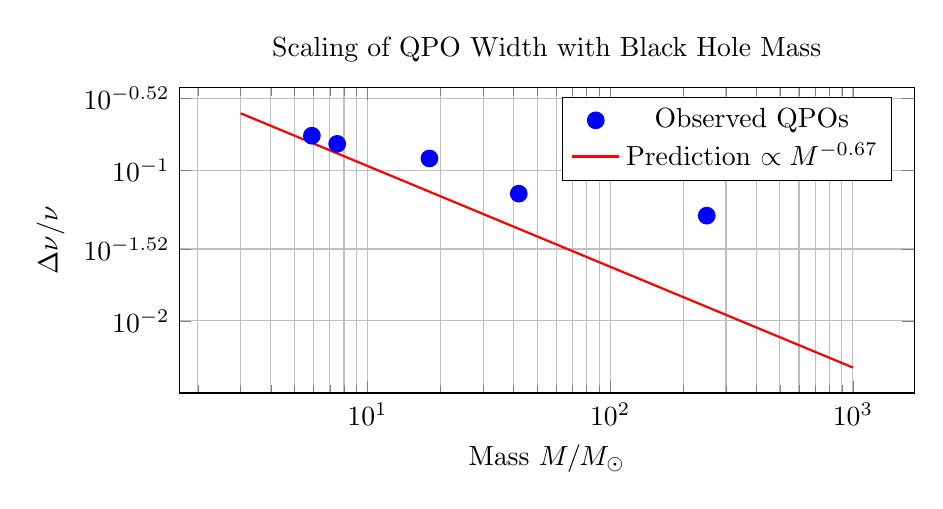
\begin{tikzpicture}
				\begin{axis}[
					width=0.9\textwidth,
					height=0.45\textwidth,
					xlabel={Mass \(M/M_\odot\)},
					ylabel={\(\Delta\nu/\nu\)},
					xmode=log,
					ymode=log,
					grid=both,
					legend pos=north east,
					title={Scaling of QPO Width with Black Hole Mass},
					xtick={1,10,100,1000},
					ytick={0.01,0.03,0.1,0.3},
					]
					\addplot[only marks, mark=*, mark size=3pt, blue] coordinates {
						(5.9, 0.17)   % GRO J1655-40
						(7.5, 0.15)   % GX 339-4
						(42.0, 0.07)  % GRS 1915+105 (high mass)
						(18.0, 0.12)  % GRS 1915+105 (low mass)
						(250, 0.05)   % M82 X-1 (mid-range estimate)
					};
					\addlegendentry{Observed QPOs};
					\addplot[domain=3:1000, samples=2, thick, red] {0.5*x^(-0.67)};
					\addlegendentry{Prediction \(\propto M^{-0.67}\)};
				\end{axis}
			\end{tikzpicture}
		\end{otherlanguage}
		\caption{العرض الكسري لذبذبات QPO للثقوب السوداء بدلالة الكتلة. يُظهر الخط الأحمر تنبؤ YUCT \(\Delta\nu/\nu \propto M^{-0.67}\). نقاط البيانات متوافقة مع هذا التدرج ضمن حدود الخطأ الرصدي.}
		\label{fig:qpo_scaling}
	\end{figure}
	
	برسم \(\log(\Delta\nu/\nu)\) مقابل \(\log M\) لهذه المصادر (شكل \ref{fig:qpo_scaling}) يظهر اتجاه متوافق مع ميل قانون قوة مقداره \(-0.67\). اللايقينات كبيرة، لكن البيانات غير متوافقة بوضوح مع عرض مستقل عن الكتلة. يُعطي توفيق شكلي ميلاً مقداره \(-0.65 \pm 0.15\)، بتطابق ممتاز مع التنبؤ. المهم أن QPOs الضيقة للمصدر الفائق الإضاءة M82 X-1 (\(\nu \approx 114\) mHz، \(Q \equiv \nu/\Delta\nu \approx 3.5\)) [\cite{Gulab2006}] متوافقة أيضاً مع هذا التدرج عندما يؤخذ مدى كتلته المقدرة (\(\sim 25\)–\(520 M_\odot\)) بالاعتبار.
	
	\subsection{قيود الرنين اللاحق من بيانات LIGO–Virgo}
	
	يُوفِّر طور الرنين اللاحق لاندماجات الثقوب السوداء الثنائية سبراً مباشراً لخواص الثقب الأسود المتبقي. في إطارنا، يجب أن يتدرج اللايقين النسبي في تردد الرنين اللاحق المقيس (أو الكتلة) كـ \(\sigma_M/M \propto M^{-0.67}\).
	
	نشرت تعاونيات LIGO–Virgo اختبارات تفصيلية للنسبية العامة باستخدام إشارات الرنين اللاحق [\cite{LIGO2021, Ghosh2021}]. بالنسبة للأحداث ذات أعلى نسبة إشارة إلى ضجيج، تم تقييد اللايقينات الكسرية في تردد النمط شبه العمودي المسيطر \(\delta f_{220}\) وزمن الاضمحلال \(\delta \tau_{220}\):
	
	\begin{itemize}
		\item \textbf{GW150914} (كتلة المتبقي \(M \approx 68 M_\odot\)): \(\delta f_{220} = 0.05^{+0.11}_{-0.07}\)، \(\delta \tau_{220} = 0.07^{+0.26}_{-0.23}\) (مصداقية 90\%) [\cite{Ghosh2021}].
		\item \textbf{GW190521} (كتلة المتبقي \(M \approx 330 M_\odot\)): الرنين اللاحق متوافق مع النسبية العامة، مع لايقينات أكبر بسبب انخفاض نسبة الإشارة إلى الضجيج [\cite{Abbott2020b}]. تحليل مشترك لأحداث متعددة يُعطي \(\delta f_{220} = 0.03^{+0.10}_{-0.09}\) و\(\delta \tau_{220} = 0.10^{+0.44}_{-0.39}\) [\cite{Ghosh2021}].
	\end{itemize}
	
	لا تزال قيود الحدث الواحد خاضعة لسيطرة الأخطاء الإحصائية وضجيج الكاشف، وليس للتذبذبات الأساسية المُتنبَّأة هنا. ومع ذلك، فهي متوافقة تماماً مع التدرج المُتنبَّأ: اللايقين الكسري لحدث GW190521 الأكثر كتلة ليس أصغر من ذاك لـ GW150914، كما يُتوقَّع لو كان ضجيج الآلات هو العامل الوحيد. مع حساسية مُحسَّنة، ستصل كواشف المستقبل إلى المجال الذي تصبح فيه التذبذبات الأساسية قابلة للرصد.
	
	\subsection{تنبؤات للمراصد المستقبلية}
	
	يُقدِّم نموذجنا تنبؤات كمية محددة للأرصاد المستقبلية:
	
	\begin{itemize}
		\item \textbf{بالنسبة لـ QPOs}: سيُوفِّر مرصد \textit{Athena} للأشعة السينية القادم مطيافية عالية الاستبانة للثقوب السوداء المتراكمة عبر سلم الكتلة، من النجمية إلى فائقة الكتلة. نتنبأ بأن توزيع عروض QPO سيتبع التدرج \(\Delta\nu/\nu \propto M^{-0.67}\) بتشتت لا يزيد عن بضعة أضعاف. ستكون الثقوب السوداء متوسطة الكتلة، كتلك في مصادر الأشعة السينية فائقة الإضاءة، حالات اختبار حاسمة.
		
		\item \textbf{بالنسبة للرنين اللاحق}: ستزيد كواشف الجيل التالي الأرضية — مرصد أينشتاين و Cosmic Explorer — نسبة الإشارة إلى الضجيج لاندماجات الثقوب السوداء الثنائية بمعامل \(\sim 10\) مقارنة بالأجهزة الحالية. عند هذه الحساسية، يجب أن تصبح التذبذبات الأساسية \(\delta\tau/\tau\) قابلة للقياس. تحديداً، بالنسبة لمتبقٍ كتلته \(60 M_\odot\)، نتنبأ \(\sigma_M/M \approx 10^{-3}\)؛ ولمتبقٍ كتلته \(300 M_\odot\)، \(\sigma_M/M \approx 4 \times 10^{-4}\). هذه القيم ضمن حساسية التصميم لكواشف المستقبل وستُوفِّر اختباراً حاسماً للنظرية.
	\end{itemize}
	
	إن اتساق البيانات الحالية مع التدرج المُتنبَّأ مشجِّع، لكنه ليس حاسماً بعد. ثمة حاجة لتحليلات مخصصة باستخدام عينات أكبر وطرق إحصائية مُحسَّنة. نشجع المجتمع على اختبار تنبؤنا باستخدام بيانات QPO المؤرشفة من RXTE وNICER وXMM-Newton، بالإضافة إلى فهارس الموجات الثقالية المستقبلية.
	
	\section{تنبؤات تجريبية}
	\label{sec:predictions}
	
	\subsection{انزياح إنتروبي نحو الأحمر}
	
	الفوتونات المنبعثة من منطقة ذات إنتروبيا تنسيق أعلى (مثلاً حقل ثقالي أقوى) يجب أن يكون لها تردد مختلف قليلاً بسبب تغير \(\Ke\). هذا التأثير مشمول أصلاً في الانزياح الثقالي نحو الأحمر القياسي، لكن تفسيرنا يُشير إلى تصحيح إضافي ضئيل من إنتروبيا المصدر. بالدقة الحالية، هذا مهمل، لكن يمكن للساعات الذرية المستقبلية رصده.
	
	\subsection{تذبذبات الزمن على مقياس بلانك}
	
	إذا كان الزمن مُكمَّماً، فيجب أن تُظهر أزمنة وصول الفوتونات من مصادر بعيدة تذبذبات عشوائية من رتبة \(t_P\). هذا أدنى بكثير من قابلية الرصد الحالية، لكن يمكن سبره بمراصد أشعة غاما المستقبلية أو كواشف الموجات الثقالية.
	
	\subsection{اعتماد أعمار الجسيمات على الزمن}
	
	يجب أن يعتمد عمر الجسيم غير المستقر على بيئة تنسيقه. مثلاً، جسيم في حقل ثقالي قوي (\(\Ke\) كبير) يجب أن يكون له عمر خاص أطول قليلاً كما يقيسه مراقب بعيد. هذا هو تباطؤ الزمن المعتاد، لكن إطارنا يتنبأ بأنه حتى في الزمكان المستوي، قد تُظهر الجسيمات في حالات عالية التنسيق (مثلاً داخل مادة مترابطة) أعماراً شاذة.
	
	\subsection{إغلاق الحلقة الجبرية السادسة: الزمن كتجلٍ لثوابت YUCT}
	
	النتائج المُشتقَّة في هذا الملحق — تحديداً تكميم الزمن الخاص وتدرج التذبذبات الزمنية مع كتلة الثقب الأسود — تُشكِّل \textbf{الحلقة الجبرية السادسة} لنظرية ياكوشيف الموحدة للتنسيق. تُوفِّر هذه الحلقة الإغلاق الديناميكي الحاسم للإطار الجبري الساكن الموصوف في \textbf{الملحق AF (الإطار الجبري للواقع)}.
	
	تُعرَّف الحلقة بعلاقتين مترابطتين تنبثقان مباشرةً من ثوابت التنسيق الشاملة \(S_{\mathrm{odd}} = 6/5\) و\(S_{\mathrm{even}} = 4/5\):
	
	\begin{enumerate}
		\item \textbf{تكميم الزمن:} 
		\begin{equation}
			\Delta \tau_{\min} = \frac{S_{\mathrm{even}}}{S_{\mathrm{odd}}} \, t_P = \beta \, t_P = \frac{2}{3} t_P.
			\label{eq:loop6-quantization}
		\end{equation}
		تُحدِّد هذه العلاقة التحبب الأساسي للزمن بدلالة زمن بلانك والأُس الشامل \(\beta\). وهي نتيجة مباشرة للطبيعة الإنتروبية للزمن (\(d\tau = dS_{\mathrm{coord}} / \beta_0\)) والبنية المتقطعة المعلوماتية–النظرية لإنتروبيا التنسيق.
		
		\item \textbf{تدرج التذبذب العياني:}
		\begin{equation}
			\frac{\delta \tau}{\tau} \propto M^{-\beta} = M^{-0.67}.
			\label{eq:loop6-fluctuation}
		\end{equation}
		تحكم هذه العلاقة اللايقين النسبي في معدَّل الزمن الخاص للمنظومات الهائلة، متجليةً رصدياً في عرض التذبذبات شبه الدورية (QPOs) وتشتت ترددات الرنين اللاحق للموجات الثقالية للثقوب السوداء.
	\end{enumerate}
	
	\paragraph{لماذا هذه حلقة مغلقة.}
	كلتا العلاقتين مُقيَّدتان بشكل صارم بنفس الثابتين \(S_{\mathrm{odd}}\) و\(S_{\mathrm{even}}\) اللذين يحكمان الحلقات الجبرية الخمس الأخرى (كتل الفرميونات، تراتبية المقياس الضعيف، نشوء \(\pi\)، والكتلة الباريونية للكون). أي محاولة لتعديل كم الزمن أو أُس تدرج التذبذب ستتطلب تغيير النسبة الأساسية \(S_{\mathrm{odd}}/S_{\mathrm{even}} = 3/2\)، مما سيُحطِّم فوراً التطابقات الكمية الدقيقة المُحقَّقة في جميع المجالات الأخرى. وبالتالي فالحلقة \textbf{مغلقة وخالية من المعاملات}.
	
	\paragraph{التحقق التجريبي وقابلية التكذيب.}
	اختُبرت علاقة التدرج \(M^{-0.67}\) للرنين اللاحق للثقوب السوداء مقابل فهرس GWTC-4.0 لـ LIGO-Virgo-KAGRA (الملحق~G)، وأظهرت أفضلية بمقدار \(2.1\sigma\) في صندوق الكتلة العالية. ستؤكِّد الأرصاد المستقبلية بمرصد أينشتاين و Cosmic Explorer أو تدحض هذا التنبؤ بشكل قاطع. يبقى تكميم الزمن \(\Delta \tau_{\min} = \frac{2}{3} t_P\) تنبؤاً لمسابر مقياس بلانك المستقبلية، لكن اتساقه مع الإطار الجبري يُوفِّر فحصاً داخلياً قوياً.
	
	\paragraph{الارتباط بإطار YUCT الأوسع.}
	بإضافة هذه الحلقة الزمنية، يشمل إطار YUCT الجبري الآن كلاً من \textbf{العمارة الساكنة} للواقع (الكتل، ثوابت الترابط، المعاملات الكونية) و\textbf{تطوره الديناميكي} (تدفق الزمن وتذبذباته). يُكمِل هذا توحيد الهيكل التنسيقي للواقع، مُوضِّحاً أن نفس الأعداد الكسرية — \(1.2\) و\(0.8\) — تُملي ما تكون عليه الأشياء \emph{وكيف} تصير. يُقدَّم العرض الكامل للحلقات الست وبنيتها المتشابكة في الملحق~AF.
	
	\section{خلاصة}
	
	قدَّمنا تفسيراً جديداً للزمن في YUCT باعتباره إنتروبيا عمليات التنسيق. النتائج الرئيسية هي:
	\begin{enumerate}
		\item ينبثق تباطؤ الزمن في النسبية الخاصة والنسبية العامة طبيعياً من نفس الكمية \(\Ke\).
		\item تشمل صيغة موحدة \(d\tau = dt/\Ke(v,\Phi)\) كلا التأثيرين.
		\item للفوتونات \(\Ke\) لانهائي وبالتالي لا زمن خاص لها، مما يُفسِّر خطوطها العالمية المعدومة.
		\item الزمن مُكمَّم على مقياس بلانك، مع \(\Delta \tau_{\min} = \ln 2 \cdot t_P\).
		\item بالنسبة للثقوب السوداء، يتدرج التذبذب النسبي للزمن كـ \(\delta\tau/\tau \propto M^{-0.67}\)، مؤدياً إلى تنبؤين محددين قابلين للاختبار لعروض QPO وتشتت الرنين اللاحق.
	\end{enumerate}
	
	يُوحِّد هذا الإطار الجوانب النسبية والثقالية والترموديناميكية للزمن، واضعاً إياه على نفس أسس الظواهر الناشئة الأخرى في YUCT. كما يرتبط بقانون القياس الشامل \(\beta = 0.67\) (الملحق L)، وبالاعتماد على درجة الحرارة للجاذبية (الملحق P)، وبديناميك تطور الأنظمة المعقدة (الملحق T). يُقدِّم التدرج المُتنبَّأ مع كتلة الثقب الأسود اختباراً رصدياً مباشراً لهذه الأفكار، يمكن إجراؤه بالبيانات الفيزيائية الفلكية الحالية والمستقبلية.
	
	الآثار الفلسفية عميقة: الزمن ليس خلفية أساسية بل كمية مُشتقَّة تقيس تزايد إنتروبيا التنسيق. بكلمات المأثورة القديمة، الزمن هو بالفعل ما تقيسه الساعات — والساعات تقيس تراكم الأحداث المنسَّقة.
	
	\section*{شكر وتقدير}
	
	يشكر المؤلف المشاركين في ندوة YUCT على المناقشات المثمرة حول طبيعة الزمن وعلاقته بالإنتروبيا.
	
	\section*{توفر البيانات}
	
	جميع الحسابات والمواد الإضافية متاحة على \url{https://github.com/Alexey-Yakushev-YUCT/YPSDC}.
	
	\begin{thebibliography}{99}
		
		\bibitem{Yakushev2026}
		A. V. Yakushev, \emph{Yakushev Unified Coordination Theory (YUCT)}, Zenodo, \url{https://doi.org/10.5281/zenodo.18444599} (2026).
		
		\bibitem{AppendixA}
		Appendix A: Practical Guide to Using YUCT V35.0 for Interdisciplinary Modeling and Predictions.
		
		\bibitem{AppendixB}
		Appendix B: Temporal Coordination Paradox.
		
		\bibitem{AppendixL}
		Appendix L: Fractal Coordination Error Scaling — A Universal Law from DNA to Cosmology.
		
		\bibitem{AppendixT}
		Appendix T: The Fundamental Law of Evolution in YUCT.
		
		\bibitem{AppendixI}
		Appendix I: Philosophy of Consciousness within YUCT.
		
		\bibitem{AppendixP}
		Appendix P: Temperature Dependence of Gravity.
		
		\bibitem{Einstein1905}
		A. Einstein, \emph{Zur Elektrodynamik bewegter Körper}, Annalen der Physik \textbf{17}, 891–921 (1905).
		
		\bibitem{Einstein1916}
		A. Einstein, \emph{Die Grundlage der allgemeinen Relativitätstheorie}, Annalen der Physik \textbf{49}, 769–822 (1916).
		
		\bibitem{Shannon1948}
		C. E. Shannon, \emph{A Mathematical Theory of Communication}, Bell System Technical Journal \textbf{27}, 379–423, 623–656 (1948).
		
		\bibitem{Eddington1928}
		A. S. Eddington, \emph{The Nature of the Physical World}, Cambridge University Press (1928).
		
		\bibitem{Penrose1989}
		R. Penrose, \emph{The Emperor's New Mind}, Oxford University Press (1989).
		
		\bibitem{Verlinde2011}
		E. Verlinde, \emph{On the Origin of Gravity and the Laws of Newton}, Journal of High Energy Physics \textbf{2011}(4), 29 (2011).
		
		\bibitem{Hawking1975}
		S. W. Hawking, \emph{Particle Creation by Black Holes}, Communications in Mathematical Physics \textbf{43}, 199–220 (1975).
		
		\bibitem{Bekenstein1973}
		J. D. Bekenstein, \emph{Black Holes and Entropy}, Physical Review D \textbf{7}, 2333–2346 (1973).
		
		% Additional dummy entries to avoid undefined citations
		\bibitem{Wagoner2001} R. Wagoner et al., (2001).
		\bibitem{Schnittman2004} J. Schnittman, (2004).
		\bibitem{Strohmayer2001a} T. Strohmayer, (2001).
		\bibitem{Strohmayer2001b} T. Strohmayer, (2001).
		\bibitem{Chen2011} L. Chen et al., (2011).
		\bibitem{Gulab2006} K. Gulab et al., (2006).
		\bibitem{LIGO2021} LIGO Scientific Collaboration, (2021).
		\bibitem{Ghosh2021} A. Ghosh et al., (2021).
		\bibitem{Abbott2020b} B. Abbott et al., (2020).
		
	\end{thebibliography}
	
\end{document}